\begin{figure}[h] 
\centering 
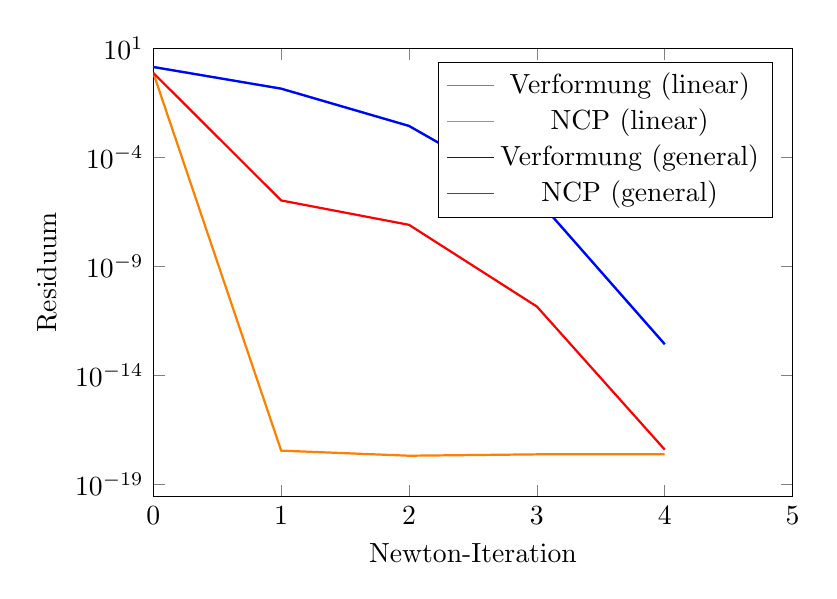
\begin{tikzpicture}[every plot/.append style={thick}] 
\begin{axis}[ 
label style={font=\normalsize}, 
xlabel={Newton-Iteration}, 
ylabel={Residuum}, 
xmin=0, xmax=5, 
ymode=log, 
ymin=0, ymax=10, 
width=0.8\textwidth, 
height=0.6\textwidth, 
legend pos=north east, 
legend style={cells={align=left}}, 
grid style=dashed, 
] 
\addplot[ 
color=cyan, 
] 
coordinates { 
(0, 1.37e+00)(1, 1.39e-01)(2, 2.72e-03)(3, 1.24e-06)(4, 2.68e-13)}; 
\addlegendentry{Verformung (linear)} 
\addplot[ 
color=orange, 
] 
coordinates { 
(0, 7.32e-01)(1, 3.50e-18)(2, 2.04e-18)(3, 2.36e-18)(4, 2.38e-18)}; 
\addlegendentry{NCP (linear)} 
\addplot[ 
color=blue, 
] 
coordinates { 
(0, 1.37e+00)(1, 1.39e-01)(2, 2.71e-03)(3, 1.23e-06)(4, 2.66e-13)}; 
\addlegendentry{Verformung (general)} 
\addplot[ 
color=red, 
] 
coordinates { 
(0, 7.32e-01)(1, 1.04e-06)(2, 7.92e-08)(3, 1.42e-11)(4, 3.90e-18)}; 
\addlegendentry{NCP (general)} 
\end{axis} 
\end{tikzpicture} 
\caption{Residuen des Stoffgesetzes 'St.Venant' mit Hinderniss 'Parabel' und 162 Freiheitsgraden für die Verschiebung.} 
\label{fiq:St.Venant_Parabel_level2} 
\end{figure} 
